%%%%%%%%%%%%%%%%%%%%%%%%%%%%%%%%%%%%%%%%%%%%%%%%%%%%%%%%%%%%%%%%%%%%%%%%%%%%%%%%%%%%%%%%%%%%%%%%%%%
%%%%%%%%%%%%%%%%%%%%%%%%%%%%%%%%%%%%%%%%%%%%%%%%%%%%%%%%%%%%%%%%%%%%%%%%%%%%%%%%%%%%%%%%%%%%%%%%%%%

\chapter{Definiciones (matem\'aticas)}

Me temo que pasar\'a alg\'un tiempo antes que esta parte sea totalmente coherente
y comprensible a un grado aceptable. Cabe mencionar
que esta fuertemente inspirada por el libro Spectral Analysis and Time Series, 
de M. Priestley \cite{Priestley81} porque est\'a expl\'icitamente dirigida a un p\'ublico 
sin trasfondo matem\'atico.

Debo citar los trabajos de Cohen, Nason, Adak, Dahlhaus, Gabor, Fryzelwicz, entre otros.
En discusiones m\'as modernas, se mencionan temas que aun no se han explorado:
ciclo-estacionariedad, procesos harmonizables, estacionariedad local y por partes,
diferencias entre memoria larga y memoria corta, espectros de ondaletas, espectros de
Wigner-Ville, Wold-Cram\'er, Gabor. 
Debo mencionarlos, pero no he trabajado en ello y no se suficiente sobre ello.

La informalidad de la redacci\'on se debe al tiempo: en versiones futuras deber\'ia mejorar.

Nota: no es prioritario, pero ser\'a una buena idea incluir una discusi\'on sobre por qu\'e
tiene sentido revisar si los EEG son estacionarios, y es que un proceso estacionario es 
b\'asicamente un ruido.

%%%%%%%%%%%%%%%%%%%%%%%%%%%%%%%%%%%%%%%%%%%%%%%%%%%%%%%%%%%%%%%%%%%%%%%%%%%%%%%%%%%%%%%%%%%%%%%%%%%

\section{Estacionariedad d\'ebil}

El ingrediente b\'asico de las series de tiempo son los procesos estoc\'asticos; para ello, se
supone dada la definci\'on de variables aleatorias, espacios de probabilidad, y espacios $L^{p}$;
si es necesario los defino, y si no me conformar\'e con citar un libro sobre series de tiempo
que cubra estos temas,
como el de Chatfield (The Analysis of Time Series: An Introduction, 2003).

Una muy buena raz\'on para empezar a describir \textbf{desde} procesos estoc\'asticos es tener
las definiciones a la mano, evitar conflictos con la notaci\'on $X(t)$ en lugar de $X_t$, y
enfatizar detalles sobre el tiempo continuo.

\begin{defn}[Proceso estoc\'astico]
Un proeso estoc\'astico $\{ X(t) \}$ es una familia de variables aleatorias indexadas por el 
s\'imbolo $t$ que pertenece a alg\'un conjunto $T \in \R$
\end{defn}

Matem\'aticamente se permitir\'a que $t$, referido como \textbf{tiempo}, tome valores 
en todo $\R$; las observaciones, en cambio,
s\'olo pueden ser tomadas en un conjunto discreto y finito de instantes en el tiempo. 
Adicionalmente, en algunas secciones se considerar\'an procesos estoc\'asticos complejos,
si bien la mayor parte del texto s\'olo usar\'a valores reales.

Esta definici\'on particular de proceso estoc\'astico deber\'ia enfatizar que para cada 
tiempo $t$, $X(t)$ es una variable aleatoria con su funci\'on de densidad de probabilidad,
sus momentos [s\'olo se consideran va's con al menos segundos momentos finitos], etc.

Otro concepto clave de este texto es el de \textbf{estaionareidad d\'ebil}; 
quiz\'a la mejor forma de motivar el adjetivo 'd\'ebil' es como contraposici\'on a 
la \textbf{estacionariedad fuerte o total}. 
Para ello, sea $F(X;\cdot)$ la funci\'on de densidad de probabilidad de $X$, es decir, 
la probabilidad de que $X\leq x$ puede expresarse como 
$
F(X;x) = P(X\leq)
$
bajo el entendido que $X$ y $x$ pueden ser vectores en $\R^{d}$.

\begin{defn}[Estacionariedad fuerte]
Un proceso estoc\'astico $\{ X(t) \}$ es fuertemente estacionario si, para cualquier 
conjunto de tiempos admisibles $t_1,t_2,\dots,t_n$ y cualquier $\tau \in \R$
se cumple que
\begin{equation*}
F\left(X(t_1),X(t_2),\dots,X(t_n);\cdot\right) 
\equiv
F\left(X(t_1+\tau),X(t_2+\tau),\dots,X(t_n+\tau);\cdot\right)
\end{equation*}
\end{defn}

La estacionariedad fuerte depende de las funciones de densidad de probabilidad conjunta para
diferentes tiempos. 
%Entre las consecuencias de que un proceso sea estacionario en el
%sentido fuerte, se encuentran:
%\begin{itemize}
%\item Media y varianzas constantes, todos los momentos constantes; es decir
%\begin{equation*}
%E[X^{n}(t)]
%\end{equation*}
%\item La funci\'on de autocorrelaci\'on s\'olo depende de 
%\end{itemize}
Si un proceso es estacionario en el sentido fuerte, entonces todas las variables $X(t)$ son 
id\'enticamente distribuidas.

%Al modelar eventos como proceso estoc\'asticos, tiene sentido que las variables aleatorias
%interfieran las unas con las otras de diversas

Con viene definir versiones menos fuertes de estacionariedad seg\'un sea posible deducirse de
las mediciones de un fen\'omeno y/o sean relevantes en su modelaci\'on.

\begin{defn}[Estacionariedad de orden $m$]
Un proceso estoc\'astico se dice estacionario de orden $m$ si, para cualquier 
conjunto de tiempos admisibles $t_1,t_2,\dots,t_n$ y cualquier $\tau \in \R$
se cumple que
\begin{equation*}
E\left[ X^{m_1}(t_1)X^{m_2}(t_2)\cdots X^{m_n}(t_n) \right]
=
E\left[ X^{m_1}(t_1+\tau)X^{m_2}(t_2+\tau)\cdots X^{m_n}(t_n+\tau) \right]
\end{equation*}
Para cualesquiera enteros $m_1,m_2,\dots,m_n$ tales que $m_1+m_2+\dots+m_n \leq m$
\end{defn}

Hay una especie de consenso seg\'un el cual la estacionariedad de orden 2, tambi\'en
llamada \textbf{estacionariedad d\'ebil} es suficiente para
que se cumplan los teoremas m\'as comunes sobre medias y varianzas.
Algunas consecuencias que un
proceso sea estacionario debilmente son las siguientes:
\begin{itemize}
\item Para todo $t$, $E[X(t)] = \mu$, una constante
\item Para todo $t$, $\Var{X(t)} = \sigma^{2}$, una constante
\item Para cualesquiera $t$, $\tau$, $\Cov{X(t+\tau),\Cov{X(t)}} = E[X(t+\tau)X(t)] - \mu^{2}$, 
una funci\'on de $\tau$ pero no de $t$
\end{itemize}

El rec\'iproco tambi\'en es cierto: si un proceso cumple las tres condiciones anteriores,
entonces es estacionario de orden 2. A su vez tres condiciones son m\'as usuales en la literatura
y tienen una intepretaci\'on m\'as clara como modelo, pues se exige que el proceso tenga media
y varianza constante, y que la funci\'on de autocorrelaci\'on no dependa de d\'onde se mida --lo
cual simplifica la estimaci\'on de estas cantidades.

Antes de proseguir, cabe mencionar que la estacionariedad fuerte se define
en t\'erminos de las funciones de densidad de probabilidad conjunta, mientras que la 
estacionariedad se define seg\'un los momentos; luego, la estacionariedad d\'ebil excluye 
procesos cuyos momentos no est\'en definidos. Por ejemplo, una colecci\'on de variables
independientes id\'enticamente distribuidos --con distribuci\'on de Cauchy-- ser\'a
fuertemente estacionario, pero no estacionario de orden $m$ para ning\'un $m$. 
%Por el contrario, un proceso estacionario de \textit{orden infinito} siempre es
%fuertemente estacionario.

Por el momento se asumir\'an procesos con segundos momentos finitos 
\textbf{debido a que} hay motivaciones
en el modelo para ello: energ\'ia finita, cambios finitos de energ\'ia, respuestas suaves, etc.

%%%%%%%%%%%%%%%%%%%%%%%%%%%%%%%%%%%%%%%%%%%%%%%%%%%%%%%%%%%%%%%%%%%%%%%%%%%%%%%%%%%%%%%%%%%%%%%%%%%

\section{El espectro de una serie de tiempo}

Quiero y me siento obligado a citar la excelente discuci\'on
filos\'ofica
de Loynes \cite{Loynes68}, resaltando la frase ''Los espectros instant\'aneos no existen''.
Tambi\'en quiero citar una discusi\'on m\'as moderna de M\'elard \cite{Melard89}, donde una
frase a favor es ''El supuesto de estacionariedad ha sido v\'alido previamente debido a la corta
duraci\'on de las series y la baja capacidad de c\'omputo''.

Pues la mayor parte de mi trabajo se ha centrado en el concepto de \textbf{espectro} de una serie
de tiempo. La mejor forma de introducir el espectro evolutivo 
--en el sentido que estoy usando-- es
presentar un proceso estacionario de orden 2,
 $\{X(t)\}$, en su representaci\'on de Cram\'er \cite{Priestley81}
[la existencia de esta representacion esta garantizada por el teorema de Khinchin-Wiener --para
procesos a tiempo continuos-- y por una extension del mismo por Wold --para procesos a tiempo
discreto.
por ahora solo cito el resultado, pero quiza sea buena idea escribir la demostracion
como apendice, una demostracion citada ya que es bastante tecnica]

\begin{equation*}
X(t) = \int_{\Lambda} A(\omega) e^{i 2\pi \omega t} dZ(\omega)
\end{equation*}

Donde el proceso $\{ Z(\omega) \}$ tiene incrementos ortogonales, es decir 
\begin{equation*}
\Cov{dZ(\omega_1,dZ(\omega_2))} = \delta(\omega_1,\omega_1) d\omega
\end{equation*}
Con $\delta$ la funci\'on delta de Dirac. Cabe mencionar que es suficiente si los incrementos
son independientes, pero se puede debilitar ese requerimiento; incluso es de notarse que no
se exige que el proceso sea al menos continuo --en el sentido estoc\'astico.

El espectro de potencia de $\{X(t)\}$ se define como

\begin{equation*}
f(\omega) = \abso{A(\omega)}^{2}
\end{equation*}

Citar\'e de Adak \cite{Adak98} una tabla donde compara varias definiciones de espectro, para
procesos no-estacionarios.

\begin{figure}[h]
\centering
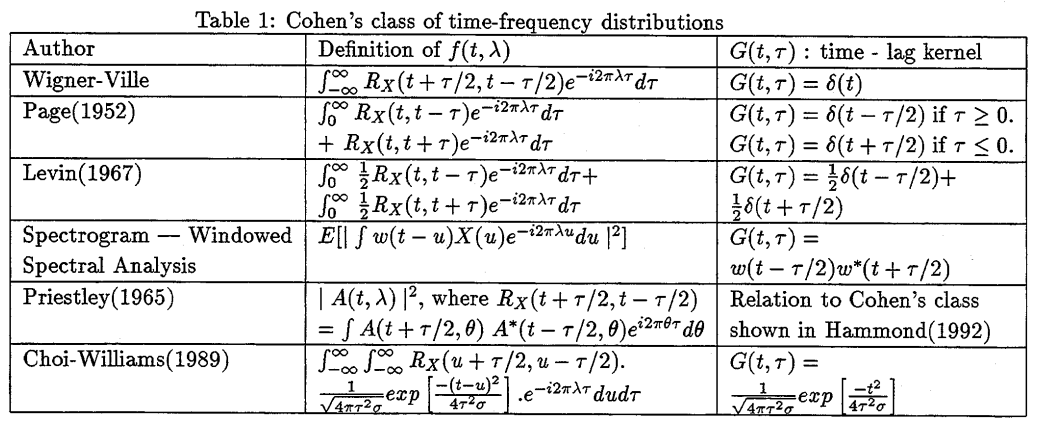
\includegraphics[width=0.9\textwidth]{tabla.png} 
\end{figure}

Dos identidades muy importantes para estimar el espectro son la \textit{equivalencia} entre
el espectro y la funci\'on de autocorrelaci\'on

\begin{equation*}
f(\omega ) = \int R_X(\tau ) e^{-i 2\pi \omega t} d\tau
\end{equation*}

Donde funci\'on de autocorrelaci\'on se ha definido como

\begin{equation*}
R_X(\tau) = E\left[ X(t) X(t+\tau) \right] = \int_0^{\infty} X(t)X(t+\tau) dt
\end{equation*}

[la demostracion es corta, batsa con reescribir una composicion de integrales como convolucion,
la incluire mas tarde]

Por otro lado, se tiene la Identidad de Parseval

\begin{equation*}
\int X^{2}(t) dt = \int f(\omega) d\omega
\end{equation*}

[esta demostracion se basa en la convergencia dominada del modulo de la integral de $X^{2}$ por
la integral del modulo (...), la incluire mas tarde]

%%%%%%%%%%%%%%%%%%%%%%%%%%%%%%%%%%%%%%%%%%%%%%%%%%%%%%%%%%%%%%%%%%%%%%%%%%%%%%%%%%%%%%%%%%%%%%%%%%%

\section{Test Priestley-Subba Rao (PSR)}

(seccion en proceso de re-redaccion)

A muy grosso modo, el test PSR estima localmente  el espectro evolutivo
 y revisa si estad\'isticamente
cambia en el tiempo.

Para ello, usa un estimador para la funci\'on de densidad espectral
que es aproximadamente (asint\'oticamente) insesgado y cuya varianza est\'a
determinada aproximadamente. La estimaci\'on se lleva a cabo en puntos en el tiempo y
la frecuencia tales que en conjunto son aproximadamente no-correlacionados.
Se aplica logaritmo para que la varianza de todos los estimadores sea aproximadamente
la misma (el logaritmo ayuda a), amen que los errores conjuntos tengan una
distribuci\'on cercana a una multinormal con correlaci\'on cero.
Finalmente se aplica una prueba ANOVA de varianza conocida.

%%%%%%%%%%%%%%%%%%%%%%%%%%%%%%%%%%%%%%%%%%%%%%%%%%%%%%%%%%%%%%%%%%%%%%%%%%%%%%%%%%%%%%%%%%%%%%%%%%%

\subsection{El espectro evolutivo}

Consid\'erese un proceso estoc\'astico a tiempo continuo $\{X(t)\}$, tal que
$E[X(t)]=0$ y $E\left[ X^{2}(t)\right] < \infty$ para todo $t$. Es decir que su media es constante
y sus segundos momentos est\'an bien definidos, aunque 
estos \'ultimos pueden cambiar con el tiempo.

Por el momento se supondr\'a que acepta una representaci\'on de la forma

\begin{equation*}
X(t) = \int_{-\pi}^{\pi} A(t ; \omega) e^{i\omega t} \, d Z(\omega)
\end{equation*}

Con $\{ Z(\omega) \}$ una familia de procesos ortogonales\footnote{De nuevo, esto implica que
$\Cov{dZ(\omega_1,dZ(\omega_2))} = \delta(\omega_1,\omega_1) d\omega$, una condici\'on m\'as
d\'ebil que la independencia} tales que

\begin{itemize}
\item $E \left[\abso{ dZ(\omega)}^{2} \right] = d\omega$
\item Para cada $t$ el m\'aximo de $A(t;\cdot)$ se encuentra en 0
\end{itemize}

Esta representaci\'on es an\'aloga a la representaci\'on de Cram\'er para un proceso
estacionario, salvo que se permite que la funci\'on $A$ cambie con el tiempo.
Siguiendo la analog\'ia, se define 
el \textbf{espectro evolutivo} de $\{X(t)\}$, con respecto a la la familia
$\mathcal{F} = \{ e^{i\omega t} A(t; \omega) \}$
 como
 
\begin{equation*}
d F(\omega;t) = \lvert A(t;\omega) \lvert^{2} d\omega
\end{equation*}

Ahora bien, si se supone que $\{X(t)\}$ es estoc\'asticametne diferenciable, entonces
se puede definir una \textbf{funci\'on de densidad espectral}

\begin{equation*}
f(t;\omega) = \lvert A(t;\omega) \lvert^{2}
\end{equation*}

Cabe destaca que si la funci\'on $A(t;\omega)$ fuera constante con respecto a $t$, se obtendr\'ia
un proceso estacionario de orden dos tal cual fue descrito en la secci\'on anterior.

%%%%%%%%%%%%%%%%%%%%%%%%%%%%%%%%%%%%%%%%%%%%%%%%%%%%%%%%%%%%%%%%%%%%%%%%%%%%%%%%%%%%%%%%%%%%%%%%%%%

\subsection{El estimador de doble ventana}

Esta t\'ecnica fue presentada por Priestley en 1965. Muy a grosso modo, es un estimador de la
funci\'on de densidad espectral con ciertas propiedades y que parte de la idea que un proceso
no-estacionario puede verse localmente como un proceso lineal generalizado.

Como meta-nota, yo empec\'e a estudiar este tipo de estimadores porque es \textit{el qeu ven\'ia
con el m\'etodo} ya que el test esta implementado en R; desde un punto de vista de difusi\'on,
es una ventaja usar un m\'etodo implementado en un software gratuito y de c\'odigo abierto --y
no una mera excusa para no explorar otros m\'etodos. En todo caso, he revisado varios otros test,
pero de momento solo este ha arrojado suficientes resultados para llenar un informe.

%{Estimador de doble ventana (Priestley, 1965 \& 1966)}
Para construir el estimador se reuieren dos funciones, $g$ y $w_T$, que servir\'an como ventanas
para extraer informaci\'on local de los datos. Debido a que sus propiedades tienen una interpretaci\'on
f\'isica desde la teor\'ia de circuitos, absorben su terminolog\'ia

\textit{
nota al pie: deberia incluir una motivacion de estos nombres,
que en parte tiene relevancia en la interpretacion. Los 
Linear Invariant Systems (LIS) suponen dependencia lineal
--constante-- respecto a todos los tiempos anteriores; 
a tiempo continuo son equivalentes a una ecuacion diferencial ordinaria lineal,
y a su vez a modelos AR. Un modelo fisico para ello son los circuitos RC, que
fueron usables en radios, y para los cuales las palabras 'filtro' y 'frecuencia'
tienen una interpretacion clara. Esta terminologia de circuitos electricos tiene sentido
para mi ya que todos los modelos de neuronas y poblaciones de neuronas que he visto hasta ahora,
por ejemplo de Ermentrout (falta citar), {Clark98,Priestley81}, PARTEN de considerar
circuitos equivalentes a los componentes neuronales, lo cual me hace pensar que es buena idea
mantener esta vision conjunta.
}

Primeramente se toma una funci\'on $g(u)$ normalizada, que en conjunto a su
transformada inversa de Fourier\footnote{Esta funci\'on 
$\Gamma(u) = \int_{-\infty}^{\infty} g(u) e^{i u \omega} du$
es referida como
\textbf{frequency-response function}, nombre tiene un poco de encanto cuando
$g$ adopta ciertas formas particulares (senos y cosenos).} 
$\Gamma$ tiene las siguientes propiedades

\begin{equation*}
2\pi \int_{-\infty}^{\infty} \lvert g(u) \lvert^{2} du 
= 
\int_{-\infty}^{\infty} \lvert \Gamma(\omega) \lvert^{2} d\omega
= 1
\end{equation*}


A partir de $g$ y $\Gamma$ se define el filtro $U$ como una convoluci\'on
con las realizaciones del proceso

\begin{equation*}
U(t,\omega) = \int_{t-T}^{t} g(u) X({t-u}) e^{i \omega (t-u)} du
\end{equation*}

Un ejemplo que est\'a en el libro de Priestley es tomar funciones del tipo

\begin{equation*}
g_h(u) = 
\begin{cases}
{1 \big{/} 2\sqrt{\pi h}} & \text{ , } \abso{u} \leq h
\\
0 & \text{ , } \abso{u} > 0
\end{cases}
\end{equation*}

Su correspondiente funci\'on de respuesta de frecuencia es complicada [me falta 
escribirla]. Es referida como la \textbf{ventana de Bartlett} y
est\'a totalmente caracterizada la siguiente propiedad

\begin{equation*}
\abso{\Gamma_h(\omega)}^{2} = \frac{1}{\pi h} \left( \frac{\text{sen} (h \omega)}{\omega} \right)^{2}
\end{equation*}

Cabe mencionar que puede entenderse al par $g$ y $\Gamma$ como ventanas en el tiempo
y las frecuencias para la serie.

---

Ahora bien, se toma una segunda ventana $W_\tau$ con las siguientes
restricciones para
su funci\'on de respuesta ante frecuencia $w_\tau$

\begin{itemize}
\item $w_{\tau}(t) \geq 0$ para cualesquiera $t$, $\tau$
\item $w_{\tau}(t) \rightarrow 0$ cuando $\lvert t \lvert \rightarrow \infty$, para todo $\tau$
\item $\displaystyle \int_{-\infty}^{\infty} w_{\tau}(t) dt = 1$ para todo $\tau$
\item $\displaystyle \int_{-\infty}^{\infty} \left( w_{\tau}(t) \right)^{2} dt < \infty$ para todo $\tau$
\item Existe una constante $C$ tal que  [T est\'a relacionado con el 'tiempo 0', pero para
tiempos de muestreo grandes se puede reemplazar por $-\infty$ EXCEPTO cerca del inicio y el final dle muestreo]
$$\lim_{\tau\rightarrow\infty} \left[ \tau \int_{t-T}^{t} \lvert W_{\tau}(\lambda) \lvert^{2} d\lambda \right] = C$$
\end{itemize}

%Ahora, si se define 
%$\displaystyle W_{T'}(\lambda) = \int_{-\infty}^{\infty} e^{-i\lambda t}w_{T'}(t) dt $

[posteriormente annadire mas detalles sobre el papel que juega el par $w_\tau$, $W_\tau$]

Como ejemplo, se puede tomar la siguiente funci\'on llamada \textbf{ventana de Daniell}

\begin{equation*}
W_\tau (t) = 
\begin{cases}
{1 \big{/} \tau} & \text{ , } -\nicefrac{1}{2} \tau \leq t \leq \nicefrac{1}{2} \tau
\\
0 & \text{ , otro caso}
\end{cases}
\end{equation*}

La cual se puede demostrar [tengo en algun lado esa demostracion]

$$\lim_{\tau\rightarrow\infty} \left[ \tau \int_{t-T}^{t} \lvert W_{\tau}(\lambda) \lvert^{2} d\lambda \right] = 2\pi$$

-----

Se define el estimador para $f_t$, con $0 \leq t \leq T$
\begin{equation*}
\widehat{f_t}(\omega) = \int_{t-T}^{t} w_{T'}(u) \lvert U(t-u,\omega) \lvert^{2} du
\end{equation*}

Fue demostrado por Priestley (1965, falta citar) que 

[aqui van las expresiones para el valor esperado y la varianza de $\widehat{f_t}$, me falta
escribirlas]

Pero, bajo varios supuesto adicionales [que me falta trascribir] se puede aproximar

\begin{equation*}
E\left[ \widehat{f_t}(\omega) \right] \sim f_t(\omega)
\end{equation*}

\begin{equation*}
\Var{\widehat{f_t}(\omega)} 
\sim 
\frac{C}{\tau} \left(f_t(\omega)\right)^{2} \int_{-\infty}^{\infty} \abso{\Gamma(\theta)}^{4} d\theta
\end{equation*}

Se advierte claramente que $\widehat{f_t}$ es unnestimados aproximadamente insesgado.
Para las ventanas de Bartlett y Daniell usadas como ejemplo, se tiene

\begin{equation*}
\Var{\widehat{f_t}} 
\sim 
\frac{4h}{3\tau} \left(f_t(\omega)\right)^{2}
\end{equation*}

Cabe mencionar que hay una expresi\'on expl\'icita para la covarianza de $\widehat{f_t}$
en para diferentes puntos en el tiempo y las frecuencias. Lamentablemente,
aun me falta escribirlas, son complicadas, y se describen situaciones bajo las
cuales estas covarianzas son negligibles; cabe destacar que TODAS las condiciones 
que se usan para aproximar son b\'asicamente las mismas, y dependen de que la distancia
entre los tiempos y las frecuencias sean tan grandes como sea posible.

------------

El \'ultimo ingrediente del test PSR es una transformaci\'on logar\'itmica
para regular la varianza, y quiza para cortar los bordes de las aproxiamciones.
Se define $Y_{i,j} = \log \left( \widehat{f_{t_i}}(\omega_j) \right)$, con las siguientes propiedades

\begin{equation*}
E\left[ Y_{i,j} \right] \thicksim \log \left( f_{t_i}(\omega_j) \right)
\hspace{4em}
\text{Var}\left( {Y\left(t,\omega\right)}\right) \thicksim \sigma^{2}
\end{equation*}

Luego as\'i, puede escribirse aproximadamente que

$$Y_{i,j} = \log \left( f_{t_i}(\omega_j) \right) + \varepsilon_{i,j}$$

donde $\varepsilon_{i,j}$ va iid tales que

$
E\left[ \varepsilon_{i,j} \right] = 0
\hspace{4em}
\text{Var}\left( \varepsilon_{i,j} \right) \sigma^{2}
$

Priestley cita que con esta informaci\'on incluso se puede considerar que los $\varepsilon_{i,j}$
siguen una distribuci\'on normal cada uno; Nason (2015, falta citar) comenta que
este supuesto no tiene por que cumplirse, y que es una popsible fuente de falsos positivos
para el test. Yo he hecho pruebas de normalidad a los datos, que incluire como anexos
mas tarde.

El test PSR \textit{per se} son tres test ANOVA --en su versi\'on en la que la varianza es conocida--
sobre si los $\varepsilon_{i,j}$ son estad\'isticamente negligibles en total, sobre el tiempo y sobre
las frecuencias. Para el fin de estudiar la estacionariedad, basta con que sean estad\'iticamente
no-negligibles sobre el tiempo.

[Por supuesto que los otros dos test tienen interpretacion: la negigibilidad total da informacion
sobre las marginales, y si estas pueden ser estimadas adecuadamente usando el estimador, si se
combina con negativo para no-estacionariedad es \textbf{efectivamente positivo} para estacionariedad
y toma una forma muy particular (proceso uniformemente modulado). Si sobre las frecuencias resulta
significativo (no-negligible) da informacion sobre la 'aeatoridad total' del proceso.
De tener tiempo, lo incluire como anexo, ya que ninguna de estas caracteristicas es estudiada :( ]

Lo detalles de la implementaci\'on en R estar\'an en la secci\'on de resultados.

%%%%%%%%%%%%%%%%%%%%%%%%%%%%%%%%%%%%%%%%%%%%%%%%%%%%%%%%%%%%%%%%%%%%%%%%%%%%%%%%%%%%%%%%%%%%%%%%%%%
%%%%%%%%%%%%%%%%%%%%%%%%%%%%%%%%%%%%%%%%%%%%%%%%%%%%%%%%%%%%%%%%%%%%%%%%%%%%%%%%%%%%%%%%%%%%%%%%%%%